\documentclass[12pt]{article}
% \usepackage{fullpage}
\usepackage{graphics,graphicx,subfig}
\usepackage{amsmath,multicol,lscape,framed,amssymb}
\usepackage{graphicx,epic,subfig,graphicx,tikz,pifont}
%\usepackage{multirow,epic}
% \usepackage{algorithmic,algorithm}
\usepackage{hyperref,hypcap}
\usepackage{natbib}%
\usepackage{longtable}
\usepackage{textcomp}%to use \textquotesingle
% \captionsetup{type=figure}
\hypersetup{
colorlinks,%
citecolor=blue,%
filecolor=black,%
linkcolor=blue,%
urlcolor=blue,
}
\usepackage{setspace}
\bibliographystyle{plain}

\bibstyle{plain}
\newcommand{\HRule}{\noindent\rule{\linewidth}{1.5pt}}
\newtheorem{alg}{Algorithm}
\newcommand{\cm}[1]{\begin{center}{\tt #1}\end{center}}
\newcommand{\hs}{{\tt hybrid-Lambda}}
\begin{document}

\title{Hybrid-Lambda: simulation of multiple merger and Kingman gene genealogies in species networks and species trees}
\author{Sha (Joe) Zhu}
\maketitle


\section{Introduction}


{\tt hybrid-Lambda} is a software package that can simulate gene trees within a rooted species network or a rooted species tree under the coalescent process. The main feature of this program is that users can choose to use the standard Kingman coalescent process, which produces bifurcating genealogies, or two other $\Lambda$-coalescent processes, which produce multifurcating genealogies. The other feature is that {\tt hybrid-Lambda} uses extended Newick formatted strings to make it easier to represent hybridization events between species.

\vspace{1cm}

\begin{center}
%
\begin{tikzpicture}[ultra thick]
\ifx\du\undefined
  \newlength{\du}
  \fi
  \setlength{\du}{2\unitlength}
% \ifx\du\undefined
%   \newlength{\du}
%   \fi
%   \setlength{\du}{2.5\unitlength}
% \draw[help lines,step=5\du] (-55\du,0\du) grid (40\du,70\du);
\draw(-55\du,0\du)--(-35\du,0\du);
\draw(-20\du,0\du)--(-10\du,0\du);
\draw(-10\du,0\du)--(-5\du,15\du);
\draw(-20\du,0\du)--(-15\du,15\du);
\draw(-15\du,15\du)--(-11\du,21.5\du);
\draw(-11\du,21.5\du)--(-15\du,25\du);
\draw(-35\du,0\du)--(-15\du,25\du);
% \draw(-55\du,0\du)--(-20\du,45\du);
\draw(-55\du,0\du)--(-35\du,25\du)--(-25\du,45\du)--(-20\du,50\du)--(-20\du,65\du);
% \draw(-10\du,50\du)--(-10\du,45\du);
\draw(0\du,22.5\du)--(-10\du,32.5\du);
\draw(-5\du,45\du)--(-10\du,32.5\du);
\draw(40\du,0\du)--(30\du,0\du);
\draw(15\du,0\du)--(0\du,0\du);
\draw(0\du,0\du)--(-5\du,15\du);
\draw(15\du,0\du)--(10\du,15\du);
\draw(10\du,20\du)--(10\du,15\du);
\draw(10\du,20\du)--(14\du,30\du);
\draw(30\du,0\du)--(14\du,30\du);
% \draw(45\du,0\du)--(10\du,45\du);
\draw(40\du,0\du)--(25\du,30\du)--(5\du,50\du)--(5\du,65\du);
% \draw(10\du,50\du)--(10\du,45\du);
\draw(0\du,22.5\du)--(5\du,35\du);
\draw(-5\du,45\du)--(5\du,35\du);
% \pgfmathsetmacro{\Xb}{random(7)};
\draw[thick](-40\du,0\du)--(-39\du,1\du)--(-39\du,2\du)--(-39\du,3\du)--(-38\du,4\du)--(-40\du,5\du)--(-40\du,6\du)--(-39\du,7\du)--(-39\du,8\du)--(-39\du,9\du)--(-39\du,10\du);
\fill(-39\du,10\du)[black]circle(2.5pt);
\fill(-15\du,50\du)[black]circle(2.5pt);
\fill(-5\du,60\du)[black]circle(2.5pt);
\fill(10\du,40\du)[black]circle(2.5pt);
\node at (-45\du,-5\du)[below]{\bf A};
\node at (-15\du,-5\du)[below]{\bf B};
\node at (7.5\du,-5\du)[below]{\bf C};
\node at (35\du,-5\du)[below]{\bf D};
\node at (-50\du,-7\du)[above]{\small a$_1$};
\node at (-45\du,-7\du)[above]{\small a$_2$};
\node at (-40\du,-7\du)[above]{\small a$_3$};
\node at (-15\du,-7\du)[above]{\small b$_1$};
\node at (5\du,-7\du)[above]{\small c$_1$};
\node at (10\du,-7\du)[above]{\small c$_2$};
\node at (35\du,-7\du)[above]{\small d$_1$};
% \draw[thick](-39\du,10\du)--(-15\du,50\du);
% \draw[thick](-15\du,50\du)--(-5\du,60\du);
% \draw[thick](10\du,40\du)--(-5\du,60\du);
% \draw[thick](35\du,0\du)--(20\du,30\du);
% \draw[thick](20\du,30\du)--(10\du,40\du);
% \draw[thick](-15\du,0\du)--(-10\du,15\du);
% \draw[thick](-10\du,15\du)--(0\du,20\du);
% \draw[thick](0\du,20\du)--(10\du,40\du);
% \draw[thick](5\du,0\du)--(0\du,15\du);
% \draw[thick](10\du,0\du)--(5\du,15\du);
% \draw[thick](0\du,15\du)--(-15\du,30\du);
% \draw[thick](-15\du,30\du)--(-15\du,50\du);
% \draw[thick](5\du,15\du)--(10\du,40\du);
\draw[thick](-39\du,10\du)--(-38\du,12\du)--(-36\du,14\du)--(-36\du,16\du)--(-35\du,18\du)--(-32\du,20\du)--(-32\du,22\du)--(-31\du,24\du)--(-30\du,26\du)--(-29\du,28\du)--(-28\du,30\du)--(-25\du,32\du)--(-24\du,34\du)--(-23\du,36\du)--(-23\du,38\du)--(-22\du,40\du)--(-20\du,42\du)--(-18\du,44\du)--(-18\du,46\du)--(-17\du,48\du)--(-15\du,50\du);
\draw[thick](-15\du,50\du)--(-15\du,51\du)--(-13\du,52\du)--(-12\du,53\du)--(-11\du,54\du)--(-10\du,55\du)--(-9\du,56\du)--(-8\du,57\du)--(-7\du,58\du)--(-7\du,59\du)--(-5\du,60\du);
\draw[thick](10\du,40\du)--(9\du,42\du)--(6\du,44\du)--(5\du,46\du)--(4\du,48\du)--(3\du,50\du)--(0\du,52\du)--(0\du,54\du)--(-1\du,56\du)--(-4\du,58\du)--(-5\du,60\du);
\draw[thick](35\du,0\du)--(34\du,2\du)--(33\du,4\du)--(32\du,6\du)--(31\du,8\du)--(30\du,10\du)--(30\du,12\du)--(29\du,14\du)--(27\du,16\du)--(26\du,18\du)--(26\du,20\du)--(24\du,22\du)--(23\du,24\du)--(23\du,26\du)--(22\du,28\du)--(20\du,30\du);
\draw[thick](20\du,30\du)--(19\du,31\du)--(18\du,32\du)--(17\du,33\du)--(15\du,34\du)--(15\du,35\du)--(14\du,36\du)--(12\du,37\du)--(13\du,38\du)--(10\du,39\du)--(10\du,40\du);
\draw[thick](-15\du,0\du)--(-15\du,1\du)--(-15\du,3\du)--(-14\du,4\du)--(-14\du,5\du)--(-13\du,7\du)--(-11\du,9\du)--(-11\du,10\du)--(-11\du,11\du)--(-12\du,12\du)--(-11\du,13\du)--(-11\du,14\du)--(-10\du,15\du);
\draw[thick](-10\du,15\du)--(-8\du,16\du)--(-6\du,17\du)--(-4\du,18\du)--(-2\du,19\du)--(0\du,20\du);
\draw[thick](0\du,20\du)--(2\du,24\du)--(3\du,26\du)--(4\du,28\du)--(5\du,30\du)--(6\du,32\du)--(8\du,34\du)--(7\du,36\du)--(10\du,38\du)--(10\du,40\du);
\draw[thick](5\du,0\du)--(5\du,1\du)--(5\du,2\du)--(3\du,5\du)--(3\du,6\du)--(2\du,7\du)--(3\du,8\du)--(2\du,10\du)--(1\du,11\du)--(2\du,12\du)--(1\du,13\du)--(1\du,14\du)--(0\du,15\du);
\draw[thick](10\du,0\du)--(10\du,1\du)--(8\du,4\du)--(7\du,5\du)--(8\du,6\du)--(8\du,7\du)--(7\du,8\du)--(7\du,10\du)--(6\du,13\du)--(5\du,14\du)--(5\du,15\du);
\draw[thick](0\du,15\du)--(-2\du,18\du)--(-5\du,19\du)--(-5\du,20\du)--(-7\du,21\du)--(-6\du,22\du)--(-8\du,23\du)--(-9\du,24\du)--(-10\du,25\du)--(-12\du,26\du)--(-12\du,27\du)--(-14\du,28\du)--(-15\du,29\du)--(-15\du,30\du);
\draw[thick](-15\du,30\du)--(-17\du,35\du)--(-16\du,40\du)--(-14\du,45\du)--(-15\du,50\du);
\draw[thick](5\du,15\du)--(5\du,17\du)--(5\du,19\du)--(7\du,21\du)--(6\du,23\du)--(6\du,25\du)--(7\du,27\du)--(7\du,29\du)--(8\du,31\du)--(8\du,33\du)--(10\du,35\du)--(10\du,37\du)--(10\du,40\du);
\draw[thick](-45\du,0\du)--(-44\du,1\du)--(-44\du,2\du)--(-43\du,3\du)--(-42\du,4\du)--(-41\du,5\du)--(-41\du,6\du)--(-40\du,7\du)--(-39\du,8\du)--(-40\du,9\du)--(-39\du,10\du);
\draw[thick](-50\du,0\du)--(-49\du,1\du)--(-48\du,2\du)--(-45\du,3\du)--(-44\du,4\du)--(-45\du,5\du)--(-44\du,6\du)--(-41\du,7\du)--(-40\du,8\du)--(-39\du,9\du)--(-39\du,10\du);
\draw[thick,->](-45\du,30\du)--(-36\du,25\du);
\node at (-45\du,30\du)[above]{\footnotesize species network};
\draw[thick,->](15\du,55\du)--(6\du,45\du);
\node at (15\du,55\du)[right]{\footnotesize gene genealogies};
\draw[thick,->](20\du,50\du)--(11\du,41\du);
\node at (20\du,50\du)[right]{\footnotesize multiple merger};
\draw[thick,->](-30\du,55\du)--(-17\du,51\du);
\draw[thick,->](-30\du,55\du)--(-7\du,60\du);
\node at (-30\du,55\du)[left]{\footnotesize binary mergers};
% \node at (-45\du,55\du)[below]{\footnotesize (or Kingman coalescent)};
% \node at (-30\du,55\du)[left]{\footnotesize multiple merger};
% \node at (-45\du,55\du)[below]{\footnotesize (or Kingman coalescent)};
\draw[thick,->](-50\du,15\du)--(-41\du,11\du);
\node at (-55\du,15\du)[above]{\footnotesize multiple merger};
\end{tikzpicture}

\begin{tikzpicture}[ultra thick]
\ifx\du\undefined
  \newlength{\du}
  \fi
  \setlength{\du}{2\unitlength}
% \ifx\du\undefined
%   \newlength{\du}
%   \fi
%   \setlength{\du}{2.5\unitlength}
% \draw[help lines,step=5\du] (-55\du,0\du) grid (40\du,70\du);
\draw(-55\du,0\du)--(-35\du,0\du);
\draw(-20\du,0\du)--(-10\du,0\du);
\draw(-10\du,0\du)--(-5\du,15\du);
\draw(-20\du,0\du)--(-15\du,15\du);
\draw(-15\du,15\du)--(-11\du,21.5\du);
\draw(-11\du,21.5\du)--(-15\du,25\du);
\draw(-35\du,0\du)--(-15\du,25\du);
% \draw(-55\du,0\du)--(-20\du,45\du);
\draw(-55\du,0\du)--(-35\du,25\du)--(-25\du,45\du)--(-20\du,50\du)--(-20\du,65\du);
% \draw(-10\du,50\du)--(-10\du,45\du);
\draw(0\du,22.5\du)--(-10\du,32.5\du);
\draw(-5\du,45\du)--(-10\du,32.5\du);
\draw(40\du,0\du)--(30\du,0\du);
\draw(15\du,0\du)--(0\du,0\du);
\draw(0\du,0\du)--(-5\du,15\du);
\draw(15\du,0\du)--(10\du,15\du);
\draw(10\du,20\du)--(10\du,15\du);
\draw(10\du,20\du)--(14\du,30\du);
\draw(30\du,0\du)--(14\du,30\du);
% \draw(45\du,0\du)--(10\du,45\du);
\draw(40\du,0\du)--(25\du,30\du)--(5\du,50\du)--(5\du,65\du);
% \draw(10\du,50\du)--(10\du,45\du);
\draw(0\du,22.5\du)--(5\du,35\du);
\draw(-5\du,45\du)--(5\du,35\du);
% \pgfmathsetmacro{\Xb}{random(7)};
\draw[thick](-40\du,0\du)--(-39\du,1\du)--(-39\du,2\du)--(-39\du,3\du)--(-38\du,4\du)--(-40\du,5\du)--(-40\du,6\du)--(-39\du,7\du)--(-39\du,8\du)--(-39\du,9\du)--(-39\du,10\du);
\fill(-39\du,10\du)[black]circle(2.5pt);
\fill(-15\du,50\du)[black]circle(2.5pt);
\fill(-5\du,60\du)[black]circle(2.5pt);
\fill(10\du,40\du)[black]circle(2.5pt);
\node at (-45\du,-5\du)[below]{\bf A};
\node at (-15\du,-5\du)[below]{\bf B};
\node at (7.5\du,-5\du)[below]{\bf C};
\node at (35\du,-5\du)[below]{\bf D};
\node at (-50\du,-7\du)[above]{\small a$_1$};
\node at (-45\du,-7\du)[above]{\small a$_2$};
\node at (-40\du,-7\du)[above]{\small a$_3$};
\node at (-15\du,-7\du)[above]{\small b$_1$};
\node at (5\du,-7\du)[above]{\small c$_1$};
\node at (10\du,-7\du)[above]{\small c$_2$};
\node at (35\du,-7\du)[above]{\small d$_1$};
% \draw[thick](-39\du,10\du)--(-15\du,50\du);
% \draw[thick](-15\du,50\du)--(-5\du,60\du);
% \draw[thick](10\du,40\du)--(-5\du,60\du);
% \draw[thick](35\du,0\du)--(20\du,30\du);
% \draw[thick](20\du,30\du)--(10\du,40\du);
% \draw[thick](-15\du,0\du)--(-10\du,15\du);
% \draw[thick](-10\du,15\du)--(0\du,20\du);
% \draw[thick](0\du,20\du)--(10\du,40\du);
% \draw[thick](5\du,0\du)--(0\du,15\du);
% \draw[thick](10\du,0\du)--(5\du,15\du);
% \draw[thick](0\du,15\du)--(-15\du,30\du);
% \draw[thick](-15\du,30\du)--(-15\du,50\du);
% \draw[thick](5\du,15\du)--(10\du,40\du);
\draw[thick](-39\du,10\du)--(-38\du,12\du)--(-36\du,14\du)--(-36\du,16\du)--(-35\du,18\du)--(-32\du,20\du)--(-32\du,22\du)--(-31\du,24\du)--(-30\du,26\du)--(-29\du,28\du)--(-28\du,30\du)--(-25\du,32\du)--(-24\du,34\du)--(-23\du,36\du)--(-23\du,38\du)--(-22\du,40\du)--(-20\du,42\du)--(-18\du,44\du)--(-18\du,46\du)--(-17\du,48\du)--(-15\du,50\du);
\draw[thick](-15\du,50\du)--(-15\du,51\du)--(-13\du,52\du)--(-12\du,53\du)--(-11\du,54\du)--(-10\du,55\du)--(-9\du,56\du)--(-8\du,57\du)--(-7\du,58\du)--(-7\du,59\du)--(-5\du,60\du);
\draw[thick](10\du,40\du)--(9\du,42\du)--(6\du,44\du)--(5\du,46\du)--(4\du,48\du)--(3\du,50\du)--(0\du,52\du)--(0\du,54\du)--(-1\du,56\du)--(-4\du,58\du)--(-5\du,60\du);
\draw[thick](35\du,0\du)--(34\du,2\du)--(33\du,4\du)--(32\du,6\du)--(31\du,8\du)--(30\du,10\du)--(30\du,12\du)--(29\du,14\du)--(27\du,16\du)--(26\du,18\du)--(26\du,20\du)--(24\du,22\du)--(23\du,24\du)--(23\du,26\du)--(22\du,28\du)--(20\du,30\du);
\draw[thick](20\du,30\du)--(19\du,31\du)--(18\du,32\du)--(17\du,33\du)--(15\du,34\du)--(15\du,35\du)--(14\du,36\du)--(12\du,37\du)--(13\du,38\du)--(10\du,39\du)--(10\du,40\du);
\draw[thick](-15\du,0\du)--(-15\du,1\du)--(-15\du,3\du)--(-14\du,4\du)--(-14\du,5\du)--(-13\du,7\du)--(-11\du,9\du)--(-11\du,10\du)--(-11\du,11\du)--(-12\du,12\du)--(-11\du,13\du)--(-11\du,14\du)--(-10\du,15\du);
\draw[thick](-10\du,15\du)--(-8\du,16\du)--(-6\du,17\du)--(-4\du,18\du)--(-2\du,19\du)--(0\du,20\du);
\draw[thick](0\du,20\du)--(2\du,24\du)--(3\du,26\du)--(4\du,28\du)--(5\du,30\du)--(6\du,32\du)--(8\du,34\du)--(7\du,36\du)--(10\du,38\du)--(10\du,40\du);
\draw[thick](5\du,0\du)--(5\du,1\du)--(5\du,2\du)--(3\du,5\du)--(3\du,6\du)--(2\du,7\du)--(3\du,8\du)--(2\du,10\du)--(1\du,11\du)--(2\du,12\du)--(1\du,13\du)--(1\du,14\du)--(0\du,15\du);
\draw[thick](10\du,0\du)--(10\du,1\du)--(8\du,4\du)--(7\du,5\du)--(8\du,6\du)--(8\du,7\du)--(7\du,8\du)--(7\du,10\du)--(6\du,13\du)--(5\du,14\du)--(5\du,15\du);
\draw[thick](0\du,15\du)--(-2\du,18\du)--(-5\du,19\du)--(-5\du,20\du)--(-7\du,21\du)--(-6\du,22\du)--(-8\du,23\du)--(-9\du,24\du)--(-10\du,25\du)--(-12\du,26\du)--(-12\du,27\du)--(-14\du,28\du)--(-15\du,29\du)--(-15\du,30\du);
\draw[thick](-15\du,30\du)--(-17\du,35\du)--(-16\du,40\du)--(-14\du,45\du)--(-15\du,50\du);
\draw[thick](5\du,15\du)--(5\du,17\du)--(5\du,19\du)--(7\du,21\du)--(6\du,23\du)--(6\du,25\du)--(7\du,27\du)--(7\du,29\du)--(8\du,31\du)--(8\du,33\du)--(10\du,35\du)--(10\du,37\du)--(10\du,40\du);
\draw[thick](-45\du,0\du)--(-44\du,1\du)--(-44\du,2\du)--(-43\du,3\du)--(-42\du,4\du)--(-41\du,5\du)--(-41\du,6\du)--(-40\du,7\du)--(-39\du,8\du)--(-40\du,9\du)--(-39\du,10\du);
\draw[thick](-50\du,0\du)--(-49\du,1\du)--(-48\du,2\du)--(-45\du,3\du)--(-44\du,4\du)--(-45\du,5\du)--(-44\du,6\du)--(-41\du,7\du)--(-40\du,8\du)--(-39\du,9\du)--(-39\du,10\du);
\draw[thick,->](-45\du,30\du)--(-36\du,25\du);
\node at (-45\du,30\du)[above]{\footnotesize species network};
\draw[thick,->](15\du,55\du)--(6\du,45\du);
\node at (15\du,55\du)[right]{\footnotesize gene genealogies};
\draw[thick,->](20\du,50\du)--(11\du,41\du);
\node at (20\du,50\du)[right]{\footnotesize multiple merger};
\draw[thick,->](-30\du,55\du)--(-17\du,51\du);
\draw[thick,->](-30\du,55\du)--(-7\du,60\du);
\node at (-30\du,55\du)[left]{\footnotesize binary mergers};
% \node at (-45\du,55\du)[below]{\footnotesize (or Kingman coalescent)};
% \node at (-30\du,55\du)[left]{\footnotesize multiple merger};
% \node at (-45\du,55\du)[below]{\footnotesize (or Kingman coalescent)};
\draw[thick,->](-50\du,15\du)--(-41\du,11\du);
\node at (-55\du,15\du)[above]{\footnotesize multiple merger};
\end{tikzpicture}
\end{center}


\section{Download and installation}
{\tt hybrid-Lambda} can be downloaded from \url{https://code.google.com/p/hybrid-sim/}. Extract the source code by executing the following command:
\cm{tar -xf hybrid-Lambda-VERSION.tar.gz.}

It is fairly standard to compile \hs~on UNIX-like systems. In the directory {\tt hybrid-Lambda-VERSION}, execute the following command:
\begin{verbatim}
$./bootstrap
$make
\end{verbatim}

{\bf Note:} The command {\tt make doxygen-run} will generate {\tt HTML} documentation of the source code.

\section{Notation}
% \section{Notations and Input/Output formats}
\subsection{Coalescent parameters}
Under the coalescent process, the waiting time for lineages to coalesce is an exponential random variable. The Kingman coalescent process allows only two lineages to coalesce at a time. Thus the mean of the waiting time for $b$ lineages to coalesce into $b-1$ lineages is $\binom{b}{2}$ per unit of time. However, for the $\Lambda$-coalescent, if the coalescent parameter $\psi$ is between 0 and 1 \citep{Eldon2006}, the rate $\lambda_{bk}$
at which $k$ out of $b$ active ancestral lineages merge is:
\begin{equation}
\label{sim_man:eqn:psi}
\lambda_{bk}=\binom{b}{k}\psi^k(1-\psi)^{b-k},\quad \psi \in (0,1).
\end{equation}
If the coalescent parameter $\alpha$ is between 1
and 2, the rate is:
\begin{equation}
\label{sim_man:eqn:alpha}
\lambda_{bk}=\binom{b}{k}\frac{B(k-\alpha,b-k+\alpha)}{B(2-\alpha,\alpha)}, \quad \alpha \in (1,2),
\end{equation}
where $B(\cdot,\cdot)$  is the beta function \citep{Schweinsberg2003}.

\subsection{Input/output formats}\label{sim_man:input}
The input file for {\tt hybrid-Lambda} is a character string that describes the relationships among species. Standard Newick format \citep{Olsen1990} is used for inputting species trees and outputting
gene trees, e.g.:
\begin{equation}
((A:t_A,B:t_B):t_{AB},C:t_C)\label{sim_man:no_root},
\end{equation}
where $t_i$ denotes the branch length from $i$ to its parent node. {\tt hybrid-Lambda} uses the values of $t_i$ to assign parameters for different inputs. In Expression \eqref{sim_man:no_root}, the interior nodes are not labelled. However, this is not essential. {\tt hybrid-Lambda} can also recognise input Newick string whose nodes are all labelled.

Extended Newick formatted strings \citep{Cardona12008,Huson2010} label all internal
nodes, and are used for inputting species networks. In the network string, the descendants of a hybrid node are recorded before the hybrid node the first time the hybrid node appears, otherwise is written as a tip node. For example,
\begin{equation}
(((B:t_B)h\#\gamma:t^{s1}_{h},A:t_A)s1:t_{s1},(h\#\gamma:t^{s2}_{h},C:t_{C})s2:t_{s2})r,\label{sim_man:ext_no_root}
\end{equation}
where $\#$ identifies the hybrid node.
\begin{center}
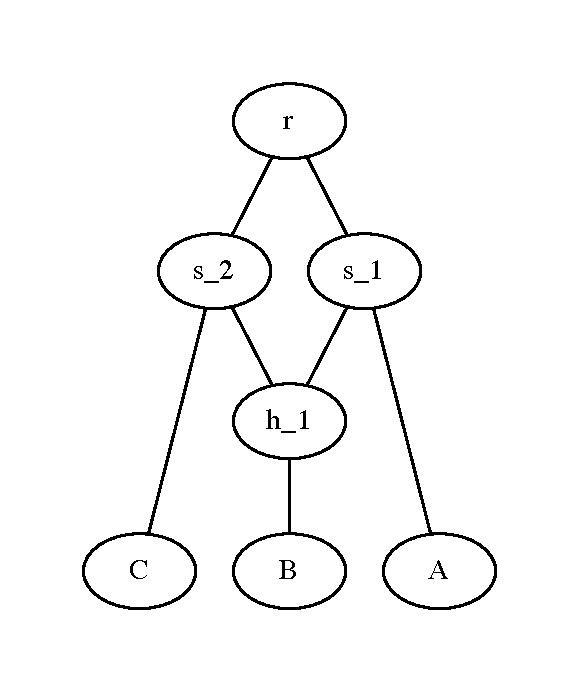
\includegraphics[height=6.5cm]{net_eg.pdf}
\end{center}
At a hybrid node, lineages travel to either parent nodes with given probabilities. The parameter $\gamma$ denotes the probability of that the lineage goes to the first parent node.
Since the hybrid node has two parent nodes, the branch length needs to be specific, i.e. $t_{i}^j$ denotes the branch length from $i$ to $j$.

Normally, standard Newick formatted and extended Newick formatted strings do not include branch lengths at the root node. However, in this program, this is required, as the input strings assign population size or the coalescent parameter at the root. Thus, Expressions \eqref{sim_man:no_root} and \eqref{sim_man:ext_no_root} are associated with Expressions \eqref{sim_man:at_root} and \eqref{sim_man:ext_at_root} respectively:
\begin{equation}
((A:t_A,B:t_B):t_{AB},C:t_C):t_{root}\label{sim_man:at_root},
\end{equation}
\begin{equation}
(((B:t_B)h\#\gamma:t^{s1}_{h},A:t_A)s1:t_{s1},(h\#\gamma:t^{s2}_{h},C:t_{C})s2:t_{s2})r:t_r.\label{sim_man:ext_at_root}
\end{equation}




\section{Commands for simulation:}
\subsection{Simulating gene trees}
\cm{\mbox{hybrid-Lambda -spcu INPUT [-num N] [-seed SEED] [-gF OUTPUT-FILE]}.}

% This is the basic command of \hs.
{\tt INPUT} is a(n) (extended) Newick formatted string (see Section \ref{sim_man:input}), which can be entered through the command line or from a text file.
%The branch lengths of the input followed by {\tt -spcu} must be in coalescent unit.
% Standard \hs~ input and output network/tree branch lengths are in coalescent unit.
If the input is followed by the flag {\tt -spcu}, its branch lengths must be in coalescent units.
The value {\tt N} following the flag {\tt -num} is the number of gene trees simulated.
% {\tt -seed} allows users to define random seed for simulation.
Users can specify a random seed for simulation by declaring it after {\tt -seed}.
By default, the branch lengths of the output trees are in coalescent units. They are saved in the file {\tt GENE\_TREE\_coal\_unit}. The flag {\tt -gF} enables the users to name the output files. For example:
\cm{\mbox{hybrid-Lambda -spcu \textquotesingle((1:1,2:1):1,3:2);\textquotesingle\  -num 3 -seed 2 -gF example1}}
will print the following message:
\begin{verbatim}
Default Kingman coalescent on all branches
Random Seed  2  used
Produced gene tree files:
example1_coal_unit
3 trees simulated.
\end{verbatim}
The following gene trees are saved in the file {\tt example1\_coal\_unit}:
\begin{verbatim}
(1_1:2.98119,(3_1:2.55301,2_1:2.55301):0.428181);
(3_1:6.66739,(2_1:1.06869,1_1:1.06869):5.5987);
(3_1:2.38966,(2_1:1.0722,1_1:1.0722):1.31746);
\end{verbatim}

\subsection{Gene tree output options and user-defined mutation rate}
\cm{\mbox{hybrid-Lambda -spcu INPUT [-gF OUTPUT-FILE] [-mu MU] [option]}}
By default, the mutation rate $\mu=0.00005$ is used. The flag {\tt -mu } makes it possible for users to define a constant mutation rate. Moreover, the options in {\tt [ ]} enable more manipulations of the output gene trees. These options include:
\begin{longtable}{lp{9cm}}
{\tt -sim\_mut\_unit }& Convert the simulated gene tree branch lengths to mutation units.\\
{\tt -sim\_num\_gener }& Convert the simulated gene tree branch lengths to number of generations.\\
{\tt -sim\_num\_mut }& Simulate the number of mutations on each branch of the simulated gene trees.\\
{\tt -sim\_Si\_num }&  Generate the file {\tt out\_table}, which includes the number of segregating sites and the total branch length of the gene tree in coalescent units.\\
\end{longtable}

For example, suppose the input network string in the file {\tt 4\_tax\_sp\_nt1\_para} is %\\{\verb ((((B:1,C:1)s1:1)h1#.5:1,A:3)s2:1,(h1#.5:1,D:3)s3:1)r; }. \\
\begin{verbatim}
 ((((B:1,C:1)s1:1)h1#.5:1,A:3)s2:1,(h1#.5:1,D:3)s3:1)r.
\end{verbatim}

\cm{hybrid-Lambda -spcu trees/4\_tax\_sp\_nt1\_para -gF example2 -num 2 \mbox{-mu 0.00003} -sim\_mut\_unit -sim\_num\_mut}
will generate the following files:
\begin{verbatim}
$ cat example2_coal_unit
((B_1:1.9099,C_1:1.9099):2.82957,(A_1:4.05317,D_1:4.05317):0.686292);
((D_1:3.77974,(C_1:1.2291,B_1:1.2291):2.55064):0.369812,A_1:4.14956);
$ cat example2_mut_unit
((B_1:0.57297,C_1:0.57297):0.848871,(A_1:1.21595,D_1:1.21595):0.205888);
((D_1:1.13392,(C_1:0.36873,B_1:0.36873):0.765192):0.110944,A_1:1.24487);
$ cat example2_num_mut
((B_1:1,C_1:1):2,(A_1:1,D_1:1):0);
((D_1:0,(C_1:1,B_1:1):0):0,A_1:3); .
\end{verbatim}

\subsection{User-defined population sizes}\label{sim_man:pop}
\cm{hybrid-Lambda -spcu INPUT-1 -pop INPUT-2}
By the default setting, the population sizes for each species are assumed to be equal and unchanged at any time, which is 10,000. This can be reassigned to other constant values followed by {\tt -pop}. As a result, the branch lengths of the gene trees in number of generations will change. This can be observed though the option {\tt -sim\_num\_gener}. For example, to simulate gene trees within a species network/tree with a population size of 25,000,
we use the following:
\cm{hybrid-Lambda -spcu INPUT -num N -pop 25000 -sim\_num\_gener.}
This command will also produce gene trees for which the branch lengths are in number of generations, saved in the file {\tt GENE\_TREE\_num\_gener}.
\newline\noindent{\bf Note:} The population size refers to the number of gene copies, not the number of individuals.

Instead of inputting a species network with branch lengths in coalescent units, input strings can have branch lengths representing the number of generations.
Moreover, in the following example, we demonstrate that if the population sizes are assumed to vary, the input strings in Expression \eqref{sim_man:at_root} can specify the population sizes on all branches and the root.
\cm{\mbox{hybrid-Lambda -spng \textquotesingle(A:50000,B:50000)r;\textquotesingle\ -pop \textquotesingle(A:50000,B:50000)r:40000;\textquotesingle.}}
%can be specified on each branch via strings in the format of expression \eqref{sim_man:at_root}, since the population size needs to be defined at the root.
% \cm{hybrid-Lambda -spng INPUT-1 -pop INPUT-2}

\subsection{Simulating multiple samples per species}
\cm{hybrid-Lambda -spcu INPUT -S n1 n2 ... }
{\tt hybrid-Lambda} sorts the taxa names in a particular order. At each character of a taxon name, it sorts:
\begin{itemize}
\item numerics in ascending order,
\item letters in alphabetical order,
\item numerics then letters,
\item upper-case letters then lower-case letters.
\end{itemize}
To sample multiple individuals, the order of the sample sizes needs to follow the order of the taxa names.

For example:
\cm{\mbox{hybrid-Lambda -spcu \textquotesingle((((A:1.1,B:1.1):2.1,a:2.2):1.1,13D:.2):.3,4:.3);\textquotesingle} \mbox{-S 2 4 3 6 5} .}
The order of the taxon names is {\tt 13D}, {\tt 4}, {\tt A}, {\tt B} and {\tt a}. Thus, the program
will sample 2 individuals in taxon {\tt 13D}, four samples from taxon {\tt 4}, three samples from taxon {\tt A}, six samples from taxon {\tt B} and five samples from taxon {\tt a}.


\subsection{Simulating gene trees with multiple merger coalescents}
\cm{hybrid-Lambda -spcu INPUT-1 -mm INPUT-2}
The Kingman coalescent is assumed by default. To use the $\Lambda$-coalescent, the coalescent parameter needs to be specified after {\tt -mm}. For details, see Equation \eqref{sim_man:eqn:psi} and \eqref{sim_man:eqn:alpha}.
Moreover, similar to assigning particular population sizes on branches (see the examples in Section \ref{sim_man:pop}), coalescent parameters can be specified as well. In this case, to assume the Kingman coalescent within some population, the multiple merger parameter needs to be set to 2. For example:
\cm{hybrid-Lambda -spcu \textquotesingle(A:1,B:1)r;\textquotesingle\ -mm \textquotesingle(A:1.9,B:.2)r:2;\textquotesingle\ -S 3 4.}


\subsection{Commands for other features:}
\subsubsection{Plot}
% \cm{ hybrid-Lambda -spcu FILENAME -dot [-branch]}
% \subsubsection{Plot by \LaTeX}
\cm{ hybrid-Lambda -spcu INPUT -dotF OUTPUT [-branch] }
{\tt hybrid-Lambda} uses the program {\tt dot} to generate figures. The option {\tt [-branch]} will label the branch lengths in the figure, e.g.:
\cm{hybrid-Lambda -spcu trees/7\_tax\_sp\_nt1\_para -dot -branch}
\begin{center}
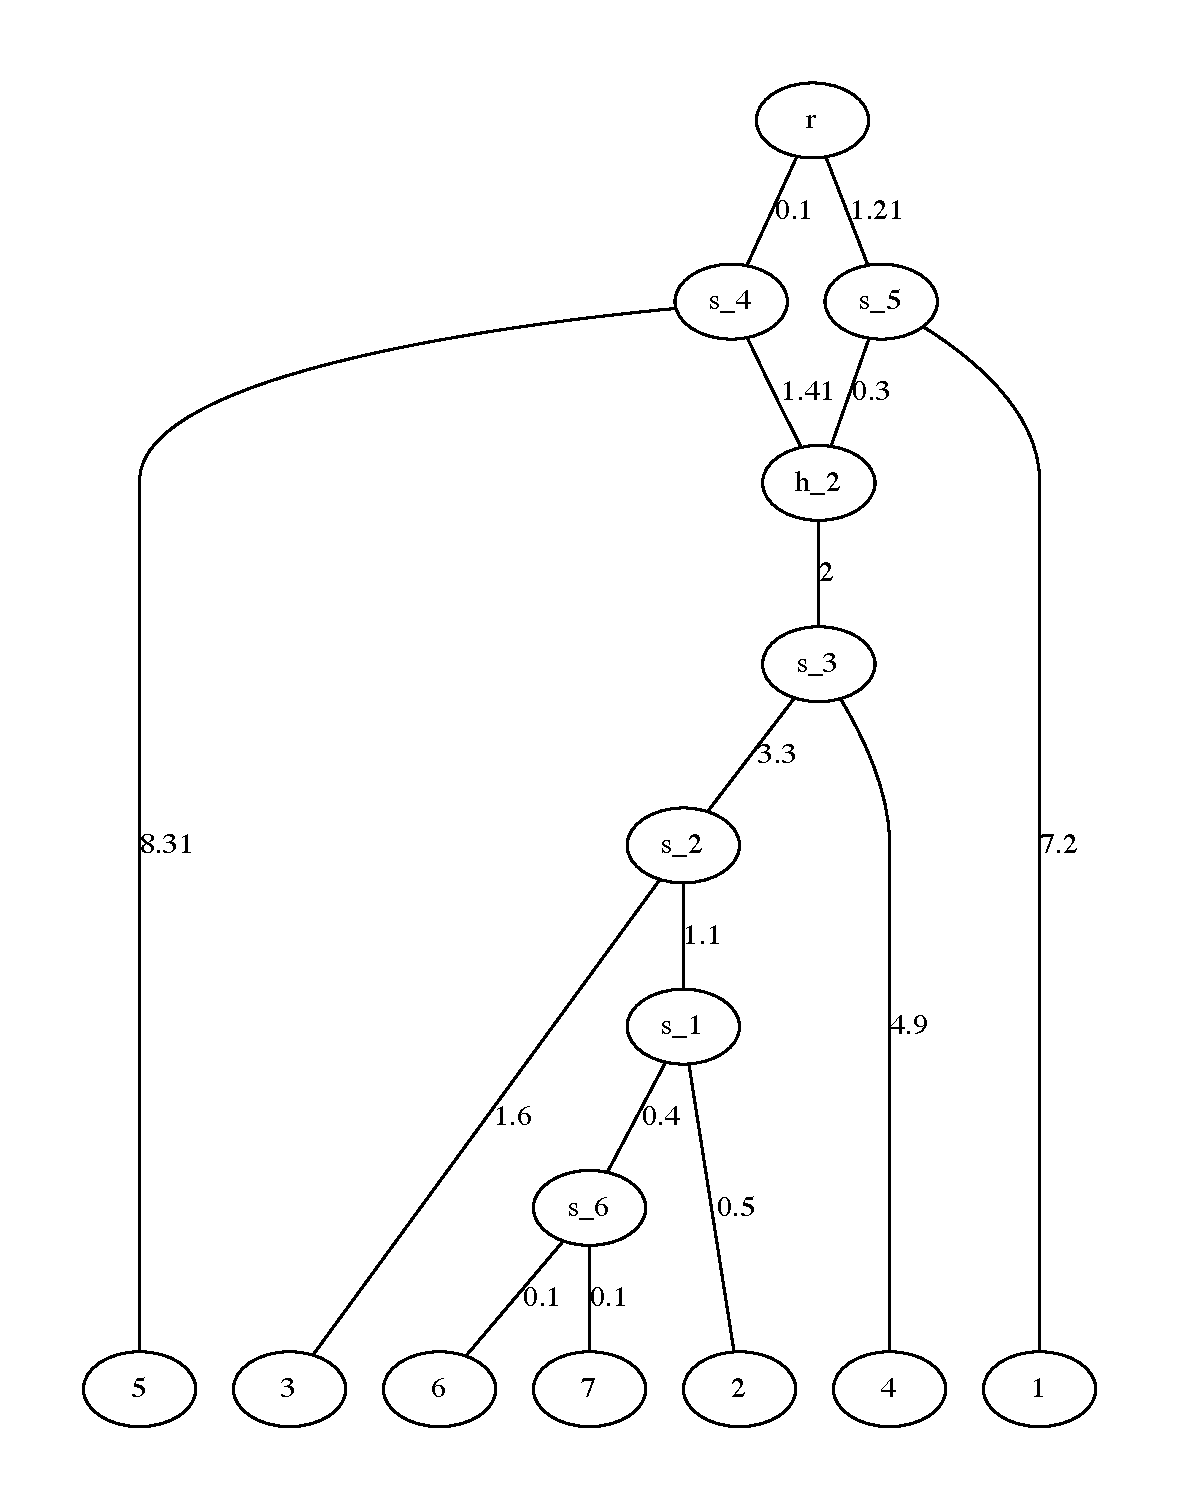
\includegraphics[width=10cm,height=10cm]{branch.pdf}
\end{center}
If the option {\tt -dot} is used instead of {\tt -dotF OUTPUT}, the figure will be saved in the file {\tt figure.pdf} by default.

Alternatively, by replacing {\tt -dotF} with {\tt plotF}, {\tt hybrid-Lambda} can generate \LaTeX\ code for plotting a network or tree.
If {\tt -plot} is used instead of {\tt -plotF OUTPUT}, the \LaTeX\ code will be saved in the file {\tt texfigure.tex} by default.
% \begin{figure}
% \centering
% \includegraphics[width=10cm]{label.pdf}%
% \end{figure}

\subsubsection{Analysing the frequencies of gene trees}
{\tt hybrid-Lambda} can generate a topology frequency table for the simulated gene trees by:
\cm{ hybrid-Lambda -spcu INPUT -num N -fF OUTPUT .}

\cm{ hybrid-Lambda -gt INPUT -fF OUTPUT}
reads trees in the file {\tt INPUT}, and generates a topology frequency table in the file {\tt OUTPUT}.
If the option {\tt -f} is used instead of {\tt -fF OUTPUT}, the analysed frequency table will be saved in the file {\tt freq\_out} by default.

\subsubsection{Simulating and analysing the monophyly topology of the gene trees}
\cm{ hybrid-Lambda -spcu INPUT-1 -S n1 n2 -mono [-mm INPUT-2]}
Recent studies on the shape of genealogies between two species investigated the probabilities of monophyletic taxa \citep{Eldon2012,Rosenberg2003}. The option {\tt -mm} generates a frequency table of the gene trees whose taxa are monophyletic in one population, both populations, or are paraphyletic and polyphyletic.
For example:
\cm{hybrid-Lambda -spcu \textquotesingle(A:5,B:5)r;\textquotesingle -mono -num 100 -mm .1 -S 4 4}
will print the following message:
\begin{verbatim}
   A mono     B mono Recip mono     A para     B para  Polyphyly
     0.02       0.01          0       0.02       0.01       0.97
Random Seed  1342238826  used
Produced gene tree files:
GENE_TREE_coal_unit
100 trees simulated.
\end{verbatim}




\section{Summary of command line options}
\begin{longtable}{lp{9cm}}
{\tt -h } or {\tt -help } &  Help. List the following content.\\
{\verb -spcu } {\tt INPUT} & Input the species network/tree string through the command line or from a file. Branch lengths of the {\tt INPUT} are in coalescent units.\\
{\verb -spng } {\tt INPUT}& Input the species network/tree string through the command line or from a file. Branch lengths of the {\tt INPUT} are in number of generations.\\
{\verb -pop } {\tt INPUT} & Population sizes are defined by a single numerical constant, or a string which specifies the population size on each branch. The string can be inputted through the command line or from a file. By default, the population size 10,000 is used.\\
{\tt -mm INPUT}  & Multiple merger parameters are defined by a single numerical constant, or a string which specifies the parameter on each branch. The string can be inputted through the command line or from a file. By default, the Kingman coalescent is used.\\
{\verb -S } {\tt n1 n2 ...} & Specify the number of samples for each taxon.\\
{\tt -num N}  & The number of gene trees to be simulated.\\
{\verb -seed } {\tt SEED} & User defined random {\tt SEED}.\\
{\tt -mu MU }  & User defined constant mutation rate $\mathbf{\mu}$. By default, a mutation rate of $0.00005$ is used.\\
{\verb -gF } {\tt FILE [option]} & Specify the filename for the simulated gene trees. \\%Define the name of file that gene trees will be saved, "GENE\_TREE" by default\\
$\qquad${\verb -sim_mut_unit }& Convert the simulated gene tree branch lengths to mutation units.\\
$\qquad${\verb -sim_num_gener } &Convert the simulated gene tree branch lengths to number of generations.\\
$\qquad${\verb -sim_num_mut }& Simulate the number of mutations on each branch of the simulated gene trees.\\
% $\qquad${\verb -sim_Si_num } & Generate the file {\tt out\_table}, which includes the number of segregating sites and the total branch length of the gene tree in coalescent unit. \\
{\verb -f } & Generate a topology frequency table for a set of input trees or simulated gene trees. The frequency table is saved in the file {\tt freq\_out} by default.\\
{\verb -fF } {\tt FILE}& The topology frequency table will be saved in {\tt FILE}.\\
{\verb -gt } {\tt FILE} & Specify the file to analyse tree topology frequencies.\\
% {\verb -seg } & Generate segregating site data\\
{\verb -mono } & Generate a frequency table of monophyletic, paraphyletic and polyphyletic trees.\\
{\tt -plot}/{\tt -dot} {\tt [option]} & Use \LaTeX ({\tt -plot}) or {\tt Dot} ({\tt -dot}) to draw the input (defined by {\tt -spcu}) network (tree).\\
$\qquad${\tt -branch}& Branch lengths will be labelled in the figure.\\
% $\qquad${\tt -label}& Branches will be labelled by post-ordered traversal.\\
{\tt -plotF}/{\tt -dotF} {\tt FILE}& The generated figure will be saved in {\tt FILE}.\\
\end{longtable}

\section*{Acknowledgements}
\paragraph{Funding:} New Zealand Marsden Fund (Sha Zhu and James Degnan), Engineering and Physical Sciences Research Council (Bjarki Eldon).  This work was partly conducted while JD was a Sabbatical Fellow at the National Institute for Mathematical and Biological Synthesis, an institute sponsored by the National Science Foundation, the U.S. Department of Homeland Security, and the U.S. Department of Agriculture through NSF Award \#EF-0832858, with additional support from The University of Tennessee, Knoxville. 
\paragraph{Included files:}C++ Mersenne twister pseudo-random number generator\citep{Matsumoto1998}.


\bibliography{article.bib}

\end{document}
  
